\documentclass[tikz,border=2pt]{standalone}
\usepackage{amsmath,amssymb}
\usepackage{pgfplots}
\pgfplotsset{compat=1.18}

\begin{document}
% LOTUS: to average g(X) you do not need the distribution of g(X); weight the values g(x)
% by the pmf of X. Here g(x) = x^2 and the pmf 0.1, 0.3, 0.4, 0.2 on -1, 0, 1, 2.
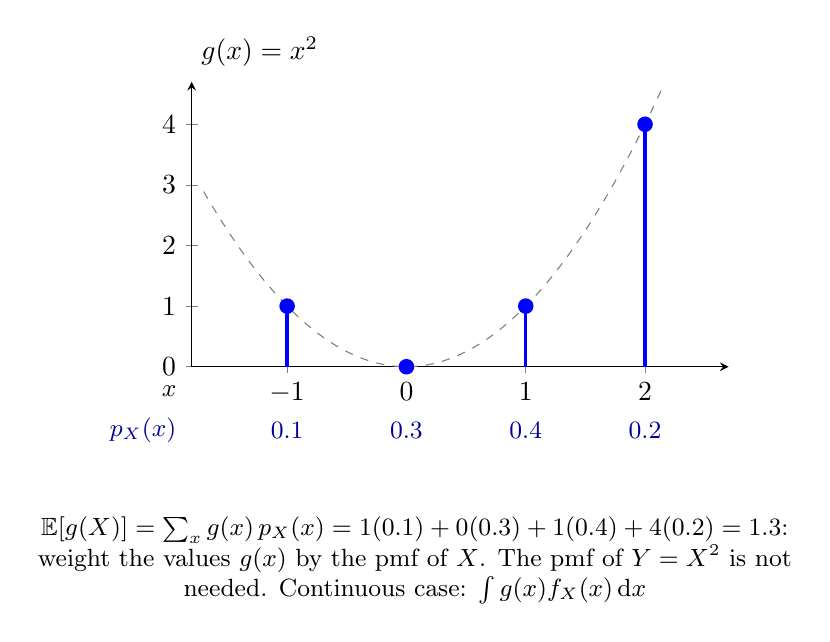
\begin{tikzpicture}
	\begin{axis}[
		axis lines=left, xmin=-1.8, xmax=2.7, ymin=0, ymax=4.7,
		xtick={-1,0,1,2}, ytick={0,1,2,3,4},
		ylabel={$g(x)=x^2$}, ylabel style={rotate=-90, anchor=south west, at={(axis description cs:0,1.02)}},
		samples=80, smooth, width=8.4cm, height=5.2cm, clip=false
		]
		\addplot[gray, dashed, domain=-1.7:2.15] {x^2};
		\addplot[ycomb, blue, very thick, mark=*, mark size=2.2pt] coordinates {(-1,1) (0,0) (1,1) (2,4)};
		\node[font=\small, anchor=east] at ([yshift=-9pt,xshift=-2pt]axis cs:-1.8,0) {$x$};
		\node[font=\small, anchor=east, blue!60!black] at ([yshift=-23pt,xshift=-2pt]axis cs:-1.8,0) {$p_X(x)$};
		\node[font=\small, blue!60!black] at ([yshift=-23pt]axis cs:-1,0) {$0.1$};
		\node[font=\small, blue!60!black] at ([yshift=-23pt]axis cs:0,0) {$0.3$};
		\node[font=\small, blue!60!black] at ([yshift=-23pt]axis cs:1,0) {$0.4$};
		\node[font=\small, blue!60!black] at ([yshift=-23pt]axis cs:2,0) {$0.2$};
	\end{axis}
	\node[anchor=north, font=\small, align=flush center, text width=9.6cm] at ([yshift=-20pt]current axis.outer south) {$\mathbb{E}[g(X)]=\sum_xg(x)\,p_X(x)=1(0.1)+0(0.3)+1(0.4)+4(0.2)=1.3$: weight the values $g(x)$ by the pmf of $X$. The pmf of $Y=X^2$ is not needed. Continuous case: $\int g(x)f_X(x)\,\mathrm{d}x$};
\end{tikzpicture}
\end{document}
